\subsection{Iterated Closest Point}\label{subsec:icp}

ICP is a technique used to align two point clouds to either create a denser one or stitch two mostly disjoint
point clouds into one.

Assuming that we have two roughly aligned points clouds $A$ and $B$, we will select a subset of matching points $A'$ and
$B'$ such that $A'_i$ corresponds to $B'_i$ (that are both close in distance and in color).
Then, we optimize the following function to find a rotation $R^*$ and a translation $t^*$ that make the matching pairs
of points overlap even more:
\[R^*, t^*=\argmin_{R,t}\sum_{i} \left\|A'_i-(RB'_i+t)\right\|_2^2\]
We then apply the found rotation and translation to update the set $B$: $B\leftarrow R^* B+t^*$.
Then, we can find a new set of matching points and repeat until convergence.

We have taken four pictures of our subject (two on the right and two on the left), rectified them
using the IPOL paper~\citep{rectification} and generated the two corresponding disparity maps using another IPOL
paper~\citep{stereomatching}.
As another preprocessing step, we removed the background of our input images manually using Apple's isolate subject
feature\footnote{\url{https://support.apple.com/en-gb/guide/photos/pht53d914053/mac}}.
Having the background in the point clouds could make the process of ICP harder, and we only require a 3D point cloud of
the subject anyway.
The results of this first step can be seen in figure~\ref{fig:icp-input}.
As we can see, the disparity maps are bad for the background, which is a non-issue.

\begin{figure}[ht]
    \centering
    \captionsetup{justification=centering}
    \begin{minipage}{.25\textwidth}
        \centering
    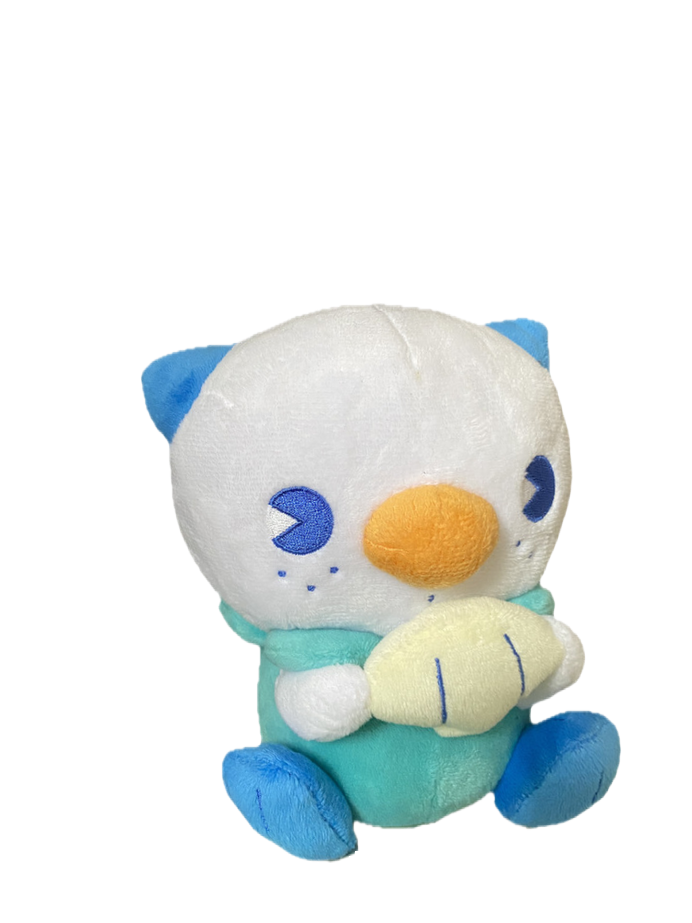
\includegraphics[width=0.95\textwidth]{assets/icp/rect_left}
    \end{minipage}%
    \begin{minipage}{.25\textwidth}
        \centering
    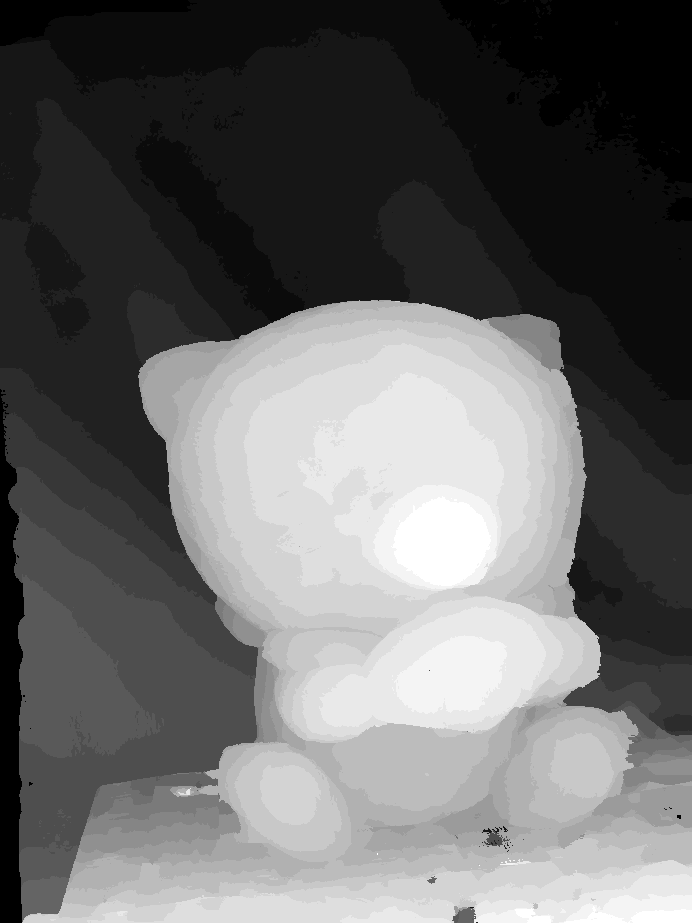
\includegraphics[width=0.95\textwidth]{assets/icp/depth_left}
    \end{minipage}%
    \begin{minipage}{.25\textwidth}
        \centering
    
\includegraphics[width=0.95\textwidth]{assets/icp/rect_right}
    \end{minipage}%
    \hfill
    \begin{minipage}{.25\textwidth}
        \centering
    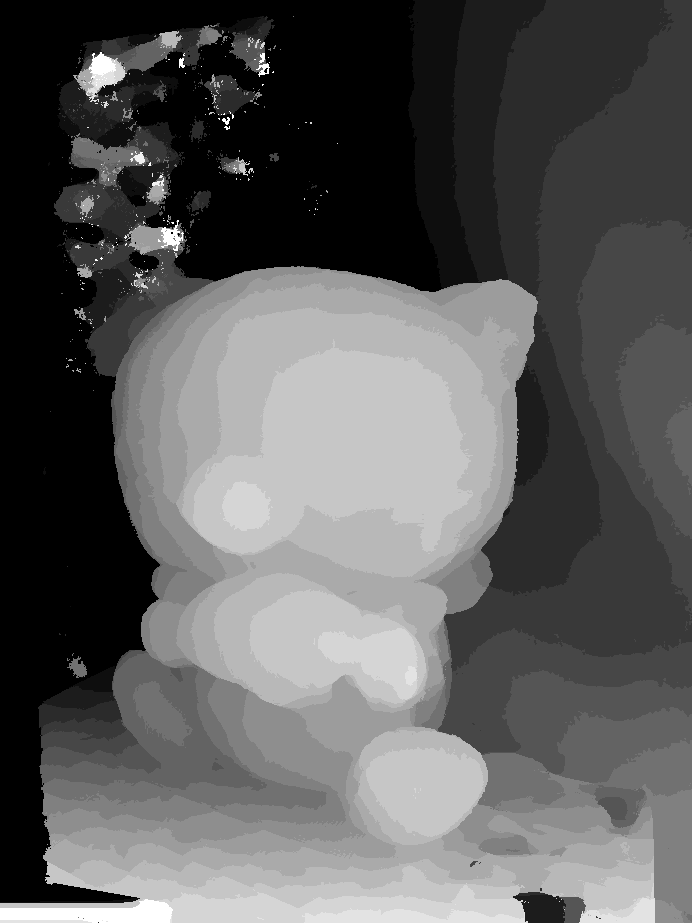
\includegraphics[width=0.95\textwidth]{assets/icp/depth_right}
    \end{minipage}
    \caption{The left and right images with their respective disparity maps.}
    \label{fig:icp-input}
\end{figure}

We can easily project points in 3D space and create a point cloud with the equations of section~\ref{subsec:rectification},
such as~\eqref{eq:disparitydepth} (with $f\approx 730$ as estimated previously).
Since the disparity maps are discrete by nature, projecting points in 3D space will create sort of a layered point
cloud, as can be seen in the leftmost image of figure~\ref{fig:icp-pcs}.

Then, using Meshlab~\citep{meshlab}, we were able to import the two point clouds, remove isolated points
and merge them using their implementation of ICP\@.
We first did a manual rough registration step by matching pairs of corresponding points to get a first alignment and
then ran the algorithm (\textit{QP.1}).
Since ICP only changes the alignment of the two point clouds, it can not change the position of each voxel individually
and the result looks like what is shown in figure~\ref{fig:icp-pcs} (middle and right images).
If we look at the middle image, we can see the two layered point clouds overlapping.
The rightmost image gives a midpoint view, which looks improvable.

\begin{figure}[ht]
    \centering
    \captionsetup{justification=centering}
    \begin{minipage}{.33\textwidth}
        \centering
    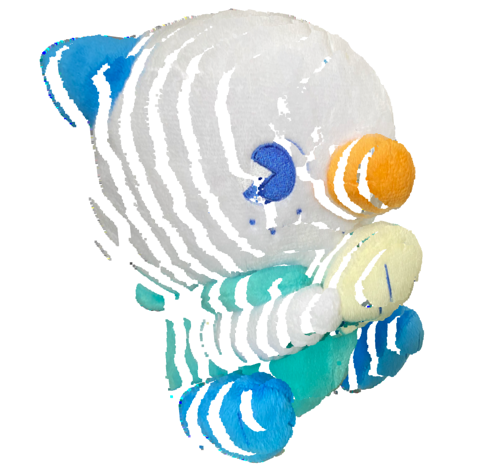
\includegraphics[width=0.95\textwidth]{assets/icp/left_pc}
    \end{minipage}%
    \begin{minipage}{.33\textwidth}
        \centering
    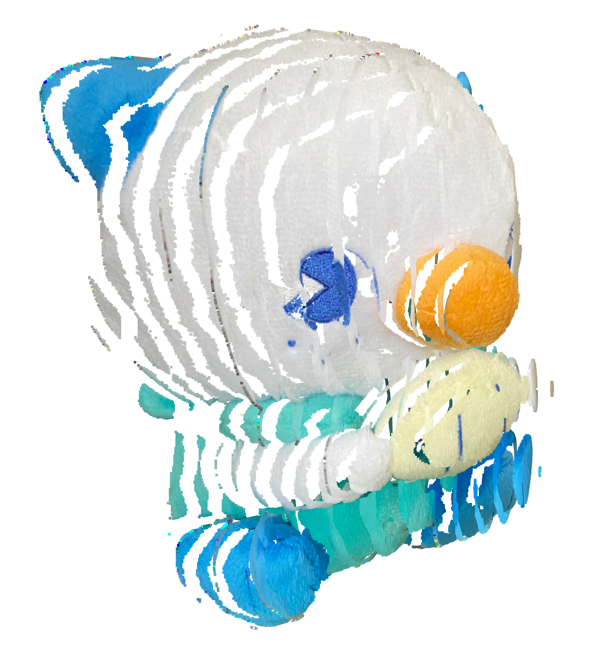
\includegraphics[width=0.95\textwidth]{assets/icp/out_left}
    \end{minipage}%
    \begin{minipage}{.33\textwidth}
        \centering
    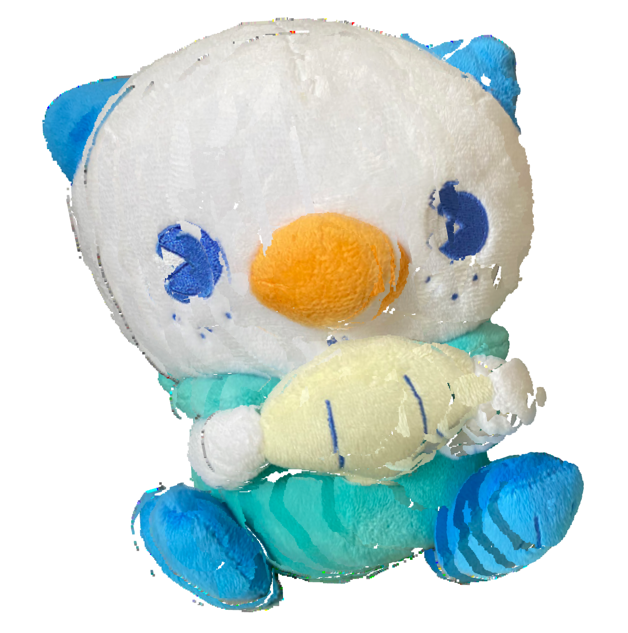
\includegraphics[width=0.95\textwidth]{assets/icp/out_mid}
    \end{minipage}
    \caption{The left image projected in 3D (left) and the final merged point cloud from the left (middle) and from
    the center (right image).}
    \label{fig:icp-pcs}
\end{figure}

To remedy the layered point cloud issue, we use a filtered version of the disparity maps generated with a bilateral
filter (with parameters found by trial and error) in order to project the images in 3D space.
This gives smoother point clouds, more suited for our purposes.
Figure~\ref{fig:icp-pcs_gaussed} shows the point cloud generated from the left input image and the final point cloud
glued using ICP in Meshlab (\textit{QP.2}).

\begin{figure}[ht]
    \centering
    \captionsetup{justification=centering}
    \begin{minipage}{.33\textwidth}
        \centering
    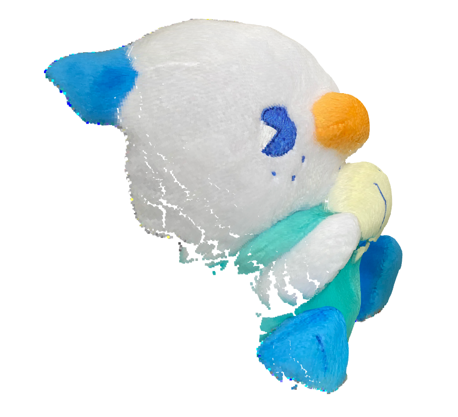
\includegraphics[width=0.95\textwidth]{assets/icp/left_pc_gauss}
    \end{minipage}%
    \begin{minipage}{.33\textwidth}
        \centering
    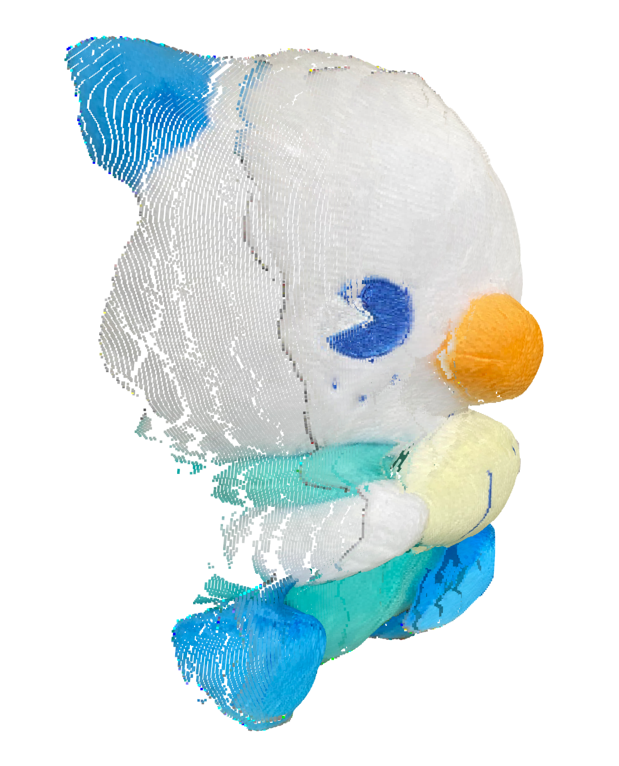
\includegraphics[width=0.95\textwidth]{assets/icp/out_gauss_left}
    \end{minipage}%
    \begin{minipage}{.33\textwidth}
        \centering
    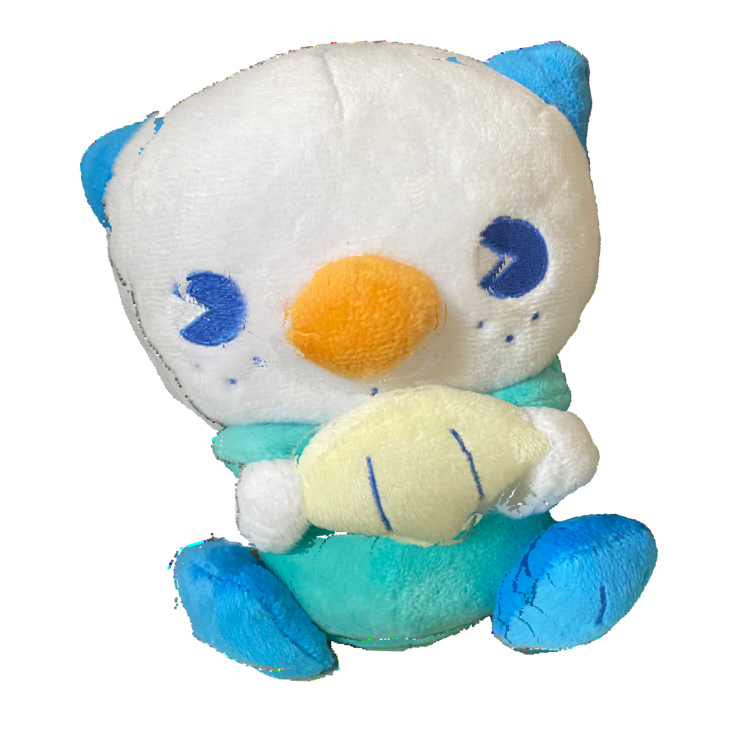
\includegraphics[width=0.95\textwidth]{assets/icp/out_gauss_mid}
    \end{minipage}
    \caption{The left image projected in 3D (left) and the final merged point cloud from the left (middle) and from
    the center (right image), generated using a filtered version of the disparity maps.}
    \label{fig:icp-pcs_gaussed}
\end{figure}

The code used for this section as well as the input images and the various point clouds (input and output to ICP) are
provided alongside this document (\textit{QP.3}).